\documentclass[11pt, a4paper]{article}
\usepackage[top=3cm,bottom=3cm,left=2.75cm,right=2cm]{geometry}
\usepackage{graphicx}
\usepackage[latin1]{inputenc}
\usepackage[spanish]{babel}
\usepackage{amsmath}

\begin{document}


\begin{figure}[t] %[h] para here [b] para bottom [t] para top
\centering

\includegraphics[width=80pt]{./logo.jpg}
\end{figure}


\begin{center}


\LARGE{UNIVERSIDAD DE BUENOS AIRES}
\Large{FACULTAD DE CIENCIAS EXACTAS Y NATURALES\\
DEPARTAMENTO DE COMPUTACI\'ON\\
\vspace{1.5cm}
ORGANIZACI\'ON DEL COMPUTADOR II\\
Segundo Cuatrimestre de 2009}

\vskip 50pt
\textbf{\Large{Procesamiento de Im\'agenes para la Detecci\'on de Bordes}}

\end{center}

\vskip 30pt

\begin{center}
\begin{tabular}{|lcl|}
\hline Integrante & LU & Correo electr\'onico \\
\hline Bianchi, Mariano & 92/08 & \texttt{bianchi-mariano@hotmail.com}\\
Brusco, Pablo & 527/08 & \texttt{pablo.brusco@gmail.com} \\
Di Pietro, Carlos Augusto Lyon & 126/08 & \texttt{cdipietro@dc.uba.ar}\\
\hline
\end{tabular}

\vspace{20 pt}

Grupo : PUNPCKHQDQ

\end{center}

\vskip 60pt

{\small
\flushleft{\textbf{Resumen}}\\
La detecci\'on de bordes es una herramienta sumamente utilizada en el procesamiento de im\'agenes, la cual permite dar mayor importancia a ciertos datos como son las l\'neas, los contornos y trazos de las mismas en detrimento de otros detalles como pueden ser matices sutiles y l\'ineas muy finas. La idea del presente trabajo es lograr implementar algoritmos de detecci\'on de bordes de im\'agenes vali\'endose para ello de los operadores m\'as comunes para tal fin. Estos son los operadores de Sobel, Prewitt y Roberts.\\
Como paso ulterior se buscar\'a comparar los resultados obtenidos con funciones an\'alogas implementadas en la librer\'ia estandar de c\'odigo abierto OpenCV. Los aspectos a comparar ser\'an tanto la calidad de resultados como el tiempo de
procesamiento medido en ciclos de reloj.\\

\vspace{22 pt}

\flushleft{\textbf{Palabras clave}}\\
Deteccion de bordes, Sobel, Roberts, Prewitt, convoluci\'on, imagenes, Lena , OpenCV.
}


\newpage



\section{Introducci\'on}

\paragraph{}
La detecci\'on de bordes es una herramienta muy utilizada dentro del \'area del procesamiento de im\'agenes. Esto se debe a que los m\'etodos de detecci\'on de bordes filtran la informaci\'on inecesaria preservando las caracter\'isticas fundamentales de la imagen, dejando por resultado una imagen que contiene toda la informaci\'on relevante de la original como son los contornos, lineas y trazos de la imagen.

\paragraph{}
En este sentido, para que un m\'etodo sea capaz de detectar un borde en necesario definir de manera no ambigua que se considera un borde. De este modo, si consideramos al pixel como la menor unidad de imagen, podr\'iamos decir que un borde se caracteriza por ser un cambio abrupto en la intensidad de pixeles vecinos.\\
Abstrayendo esta idea al plano matem\'atico, podemos caracterizar a la intensidad de los pixeles que componen la imagen como una funci\'on continua cuya representaci\'on es una curva suave salvo por picos en los cuales se produce un salto en la intensidad. Luego, para detectar un borde lo que se busca determinar son los puntos que se corresponden con los saltos de intensidad en una imagen.\\
Para ello se emplea una de las herramientas m\'as utilizadas que es el vector gradiente, el cual gr\'aficamente siempre apunta en direcci\'on a la mayor variaci\'on de la funci\'on. En nuestro an\'alisis particular, el vector gradiente act\'ua como indicador de la direcci\'on en la cual se produce la mayor variaci\'on de intensidad entre un pixel y cualquiera de sus vecinos.

\paragraph{}
Lo esperable es poder cuantificar esa m\'axima variaci\'on de intensidad entre los pixeles, razon por la cual, para cada pixel se desea determinar la norma de su vector gradiente. Se sabe por definici\'on del vector gradiente que:


$$
\nabla I = \left[ \begin{array}{l}
\vspace{11 pt}
I_x\\
I_y
\end{array}
\right]
= \left[ \begin{array}{l}
\vspace{11 pt}
\frac{\sigma I}{\sigma x}\\
\frac{\sigma I}{\sigma y}
\end{array}
\right]
$$



Luego, la norma del vector gradiente queda caracterizada por la expresi\'on:

\begin{equation}
||\nabla I|| = \sqrt{I_x ^{2}+ I_y^{2}}
\end{equation}



No obstante, para reducir la complejidad computacional, en este trabajo se opt\'o por aproximar esta norma mediante la suma de los m\'odulos de las derivadas parciales

\begin{equation}
||\nabla I|| \approx |I_x| + |I_y|
\end{equation}


En consecuencia, para calcular el gradiente de una imagen, se debe realizar previamente el c\'alculo de las derivadas parciales en cada pixel.
La forma optada en este trabajo pr\'actico para calcular dichas derivadas es mediante la aplicaci\'on de operadores dobles o de dos etapas. Los operadores utilizados, fueron los operadores de Sobel, Prewitt y Roberts. Estos operadores se caracterizan por realizar la detecci\'on de bordes en dos pasos. En el primero se buscan los bordes horizontales utilizando la m\'ascara que corresponde a la derivada parcial en X a cada pixel de la imagen. Seguidamente, y de forma an\'aloga, se buscan los bordes verticales utilizando la m\'ascara que corresponde a la derivada parcial en Y. Finalmente, para obtener todos los bordes de la imagen se suman los bordes horizontales y verticales obtenidos en el paso previo.


\paragraph{}
El objetivo de este trabajo pr\'actico es implementar un programa capaz de detectar los bordes de una imagen mediante el uso de los m\'etodos anteriormente descriptos. Se pretende que la interfaz del mismo se desarrolle en lenguaje C y que las funciones de detecci\'on de bordes se encuentren desarrolladas en lenguaje assembler.
Para la implementacion de la interfaz, se cuenta con las funciones incluidas en la librer\'ia de codigo abierto OpenCV. Esta librer\'ia provee, entre otras cosas, funciones que simplifican la carga, copia y salvado de im\'agenes, asi como tambi\'en otras funcionalidades necesarias para la realizaci\'on de este trabajo. En particular, provee tambien la funci\'on cvSobel, la cual realiza la detecci\'on de bordes de una imagen usando el operador de Sobel.
Una vez desarrollado el programa, se pretende poder comparar los m\'etodos implementados en este trabajo, con los m\'etodos provenientes de la librer\'ia de codigo abierto OpenCV. Para dicha comparaci\'on, en el caso del operador de Sobel, se har\'a uso de la funcion cvSobel anteriormente mencionada. Adem\'as, nos interesa cuantificar, la diferencia de velocidad entre las implementaciones de la librer\'ia y las del presente trabajo en funci\'on de la cantidad de ciclos de reloj necesarios para procesar una imagen.

En lo que respecta al trabajo final, el programa desarrollado es capaz de aplicar el m\'etodo de detecci\'on de bordes usando todos los operadores mencionados, dando la posibilidad de hallar bordes de toda una imagen en sus dos direcciones; mientras que en caso particular del operador de Sobel, tambi\'en brinda la opci\'on de calcular los bordes horizontales y verticales, no as\'i para los operadores de Prewitt y Roberts.

\newpage

\section{Desarrollo}

\subsection{Primera aproximaci\'on}
\paragraph{}
Para comenzar a realizar este trabajo pr\'actico lo primero que se hizo, a modo de prueba y al igual que en el trabajo anterior, fue realizar simplemente un recorrido de la imagen copiando pixel por pixel, obteniendo as\'i una copia fiel de la imagen fuente en la imagen destino. De esta modo, se aseguraba que la forma de recorrer la imagen fuese la correcta. Esto se realiz\'o porque no resultaba trivial recorrer una im\'agen de ancho m\'ultiplo de 16 de a menos pixeles.

\subsection{Implementaci\'on}
\paragraph*{}
Ya habi\'endose realizado suficientes pruebas se procedi\'o a implemetar el algoritmo deseado. Como primer paso se implement\'o la intrfaz del mismo en lenguaje C, de modo de que al ejecutar el programa por consola, este pudiera recibir como par\'ametro la imagen a procesar, asi como tambi\'en el tipo de filtro a aplicar conforme a lo pedido en el enunciado del presente trabajo.
Seguidamente se pas\'o a analizar la forma en la cu\'al se implementar\'ia cada m\'etodo. Se comenz\'o por el m\'etodo de Sobel, ya que si este m\'etodo se implementaba correctamente, el resto pod\'ia resolverse de manera an\'aloga (o en su defecto de manera muy similar).
De este modo, se busc\'o que el algoritmo de Sobel fuera recorriendo la imagen y aplicara a cada pixel la m\'ascara correspondiente, es decir la matriz de 3x3 con los valores correspondientes al operador de Sobel. A continuaci\'on se explica c\'omo se implement\'o el operador de sobel en X: una vez posicionados sobre el pixel al cual se le quer\'ia calcular la derivada, se cargaba en 3 registros xmm 3 tiras de filas adyacentes.\\
Si recordamos, el operador de sobel para X es asi:\\
\begin{table}[h]
\centering
\begin{tabular}{|c|c|c|}
\hline -1 & 0 & 1 \\ 
\hline -2 & 0 & 2 \\ 
\hline -1 & 0 & 1 \\ 
\hline 
\end{tabular}
\end{table}\\

\paragraph{}
Supongamos que las tiras de pixeles antes mencionadas, se cargaban de la siguiente manera:\\

\begin{center}
XMM0 = $\begin{array}{|c|c|c|c|c|c|c|}
\hline
S_{0,15} & S_{0,14} & S_{0,13} & \ldots & S_{0,2} & S_{0,1} & S_{0,0}\\
\hline
\end{array} $
\end{center}


\begin{center}
XMM1 = $\begin{array}{|c|c|c|c|c|c|c|}
\hline
S_{1,15} & S_{1,14} & S_{1,13} & \ldots & S_{1,2} & S_{1,1} & S_{1,0}\\
\hline
\end{array} $
\end{center}

\begin{center}
XMM2 = $\begin{array}{|c|c|c|c|c|c|c|}
\hline
S_{2,15} & S_{2,14} & S_{2,13} & \ldots & S_{2,2} & S_{2,1} & S_{2,0}\\
\hline
\end{array} $
\end{center}

donde los valores que se encuentran m\'as hacia la izquierda corresponden a los bytes m\'as significativos de los registros, y los de m\'as hacia la derecha a los menos significativos.

\paragraph{}
En el siguiente paso, se proced\'ia a sumar dichos registros, de la siguiente manera: se sumaba una vez el registro XMM0, una vez el XMM2 y finalmente dos veces el registro XMM1. Quedando dicho resultado almacenado en XMM0 de la siguiente manera:

\begin{center}
XMM0 = $\begin{array}{|c|c|c|c|c|}
\hline
S_{0,15} + 2*S_{1,15} + S_{2,15} & \ldots & S_{0,2} + 2*S_{1,2} + S_{2,2} & S_{0,1} + 2*S_{1,1} + S_{2,1} & S_{0,0} + 2*S_{1,0} + S_{2,0}\\
\hline
\end{array} $
\end{center}

Luego, se procedia a copiar este registro en alguno de los otros disponibles, y se lo shifteaba a derecha 2 bytes. Quedando asi:

\begin{center}
XMM1 = $\begin{array}{|c|c|c|c|c|}
\hline
0 & \ldots & S_{0,3} + 2*S_{1,3} + S_{2,3} & S_{0,3} + 2*S_{1,3} + S_{2,3} & S_{0,2} + 2*S_{1,2} + S_{2,2}\\
\hline
\end{array} $
\end{center}

\paragraph{}
Finalmente, se hac\'ia la resta entre XMM1 y XMM0, quedando en los 14 bytes menos significativos de XMM1 el resultado a guardar en la imagen destino.\\
En principio esto se supuso que pasaba, pero en realidad no se obtuvieron los resultados buscados. Esto se debi\'o a que cuando se hac\'ia la suma de los registros XMM0, XMM2 y 2 veces XMM1, las instrucciones usadas saturaban cada una de las sumas, pero lo que se necesitaba era que reci\'en se saturaran los valores de cada pixel una vez hecha la resta antes mencionada.

\paragraph{}
Por este motivo, lo que se realiz\'o fue hacer un desempaquetado de los datos almacenados en los registros, para que las sucesivas sumas y restas no saturaran el resultado hasta que se lo necesitaba.\\
De esta forma, se comenzaba igual que antes. Se cargaba en los registros XMM0, XMM1 y XMM2 3 tiras de pixeles de filas adyacentes, y los datos se desempaquetaban de bytes a words (s\'olo la parte baja de los mismos), quedando estos registros asi:

\begin{center}
XMM0 = $\begin{array}{|c|c|c|c|c|c|c|}
\hline
S_{0,7} & S_{0,6} & S_{0,5} & \ldots & S_{0,2} & S_{0,1} & S_{0,0}\\
\hline
\end{array} $
\end{center}


\begin{center}
XMM1 = $\begin{array}{|c|c|c|c|c|c|c|}
\hline
S_{1,7} & S_{1,6} & S_{1,5} & \ldots & S_{1,2} & S_{1,1} & S_{1,0}\\
\hline
\end{array} $
\end{center}

\begin{center}
XMM2 = $\begin{array}{|c|c|c|c|c|c|c|}
\hline
S_{2,7} & S_{2,6} & S_{2,5} & \ldots & S_{2,2} & S_{2,1} & S_{2,0}\\
\hline
\end{array} $
\end{center}

donde las posiciones que se encuentran m\'as a la izquierda son las words m\'as significativas del registro, y hacia la derecha est\'an las menos significativas.

\paragraph{}
En este punto se realizaban las mismas operaciones explicadas anteriormente, es decir, se sumaban los registros XMM0, 2 veces XMM1 y XMM2 (se almacenaba todo en XMM0) se copiaba dicha suma a XMM1, se shifteaba dicho registro, esta vez 2 words a la derecha, y se le restaba a este \'ultimo el primer registro, es decir, XMM0, quedando en las 6 words menos significativas de XMM1 los valores de los pixeles a guardar en la imagen destino. En realidad, para guardarlos en la imagen faltaba un paso m\'as. Se procedi\'o a empaquetar las words almacenadas en XMM1 a bytes. De esta forma, las words quedaban saturadas como deb\'ian (recordemos que en este punto, a\'un no se hab\'ia realizado ninguna saturaci\'on). Luego de finalizado el empaquetamiento de word a byte, se proced\'ia ahora s\'i, a guardar a donde correspond\'ia el resultado almacenado en XMM1\footnote{Para una mejor explicaci\'on del algoritmo aqu\'i descripto, se puede encontrar el pseudoc\'odigo del mismo en el anexo Pseudocodigos}.


\paragraph{}
La implementaci\'on de los dem\'as m\'etodos fue an\'aloga a la realizada anteriormente, con la \'unica diferencia de que en cada caso se realizaban otro tipo de sumas y restas, para amoldarse a la m\'ascara correspondiente, salvo en el caso de frei-chen, que al tener en la m\'ascara un valor de tipo float, los c\'alculos para dicho operador son distintos.\footnote{Este algoritmo esta explicado detalladamente en el anexo Pseudoc\'odigos}




\newpage

\section{Resultados}

\subsection{Mediciones de tiempos de ejecuci\'on}
\paragraph{}
A continaci\'on se presentan los resultados de las mediciones de ciclos de reloj de la ejecuci\'on de cada uno de los algoritmos. Asimismo se presenta una tabla comparativa de las mediciones de ciclos de reloj de cvSobel y la funci\'on an\'aloga realizada en este trabajo.\\
Por otra parte, las im\'agenes resultantes del procesamiento de bordes, que bien podr\'ian ir en esta secci\'on del informe, se encuentran al final del mismo presentadas como anexos para favorecer su visualizaci\'n.

\paragraph{}
El criterio para obtener los resultados de esta secci\'on fue realizar unas 1000 iteraci\'ones, y quedarnos con el menor tiempo arrojado por cada una de las funciones, tanto para las realizadas en este trabajo, como para las incluidas en la librer\'ia OpenCv.

\vspace{1cm}

\begin{table}[ht] %ubicacion de la tabla
\centering %centra la tabla
\begin{tabular}{|l|r|r|r|r|r|r|}
\hline
M\'etodo & Roberts & Prewitt & SobelX & SobelY & SobelXY & Frei-Chen \\
\hline
TP1A & 10926996 & 11055936 & 9117708 & 7862676 & 15924036 & --- \\
\hline
TP1B & 697272 & 2294244 & 1467132 & 1452480 & 2368380 & ???\\
\hline
\end{tabular}

\caption{Tabla comparativa de mediciones de ciclos de reloj para cada uno de los algoritmos de detecci\'on de bordes implementados en ambos trabajos pr\'acticos} %titulo de la tabla
\label{Tiempo metodos} %con esto puedo referenciar a la tabla \ref{Tiempo metodos}
\end{table}
\vspace{30pt}

\begin{table}[ht] %ubicacion de la tabla
\centering %centra la tabla
\begin{tabular}{|l|r|r|r|}
\hline
Metodo & SobelX & SobelY & SobelXY \\
\hline
TP1A & 9117708 & 7862676 & 15924036 \\
\hline
TP1B & 1467132 & 1452480 & 2368380 \\
\hline
OpenCv & 21603888 & 19262892 & 20204124 \\
\hline



\end{tabular}

\caption{Tabla comparativa de mediciones de ciclos de reloj entre los algoritmos de deteccion de bordes basados en el operador de Sobel de la libreria OpenCV y los implementados en ambos trabajos pr\'acticos} %titulo de la tabla
\label{Tiempo comparacion} %con esto puedo referenciar a la tabla \ref{Tiempo metodos}
\end{table}


\newpage
\section{Debate}
\paragraph{}
Como podemos observar en los datos obtenidos en la secci\'on de resultados, hay una clara diferencia en los ciclos de reloj necesarios para procesar una imagen entre el m\'etodo utilizado para el TP1 y el utilizado para el presente trabajo. Esto puede deberse a varios motivos, pero el principal y m\'as trivial de todos es que gracias a haber utilizado instrucciones SSE, se pudieron procesar de a m\'as de un pixel por vez haciendo aqu\'i la mayor diferencia. Adem\'as, la saturaci\'on del valor de los pixeles se realizaba automaticamente, tambi\'en gracias a las instrucciones antes mencionadas. Por lo tanto, el tiempo necesario para procesar una imagen se ve reducido ampliamente.

\paragraph{}
No obstante, la utilizaci\'on de instrucciones SSE para la mejora de ciertos puntos de un algoritmo puede ser una desventaja. Esto se debe a que no todos los procesadores tienen el mismo set de instrucciones, por lo cu\'al un algoritmo que funcione de manera excelente en una computadora, puede no comportarse como se espera en otra o directamente no funcionar.


\section{Conclusi\'ones}

\paragraph{}
Si observamos m\'as detalladamente los datos obtenidos, podremos ver grandes diferencias entre los tiempos de ejecuci\'on de la implementaci\'on anterior (TP1) y la nueva (TP2). Esto se debe a que, gracias al haber utilizado instrucciones SSE, en cada ciclo se pudieron procesar de a varios pixeles a la vez, en contraposici\'on con el trabajo pr\'actico anterior, en el cual s\'olo se pod\'ia procesar de a un pixel por vez.

\paragraph{}
Otro punto interesante es observar como se produce la saturaci\'on de un pixel. En el trabajo anterior, para poder saturar el valor obtenido para cada pixel, se deb\'ia hacer una funci\'on aparte. Esto conllevaba a un tiempo de ejecuci\'on mayor, ya que se deb\'ian hacer algunas comparaciones y asignaciones de acuerdo a si correspond\'ia saturar a 0 o a 255.\\
En el caso de este trabajo, esto era autom\'atico, por lo cual se redujeron ampliamente los tiempos de ejecuci\'on en lo que respecta al tema de saturaci\'on. 

\paragraph{}
Como conclusi\'on final, podemos decir que conociendo mejor las virtudes de un procesador se puede mejorar a\'un m\'as el tiempo de ejecuci\'on de un algoritmo realizado en lenguaje assembler. Sin embargo, se debe conocer con detalle las m\'aquinas en donde se piensa utilizar este software ya que puede no funcionar como debe, dependiendo el hardware que se utilice.


\newpage
\section{Anexo I}
\subsection{Imagenes resultantes del procesamiento de detecci\'on de bordes}

\vspace{2cm}

\begin{figure}[ht] %[h] para here [b] para bottom [t] para top
\centering
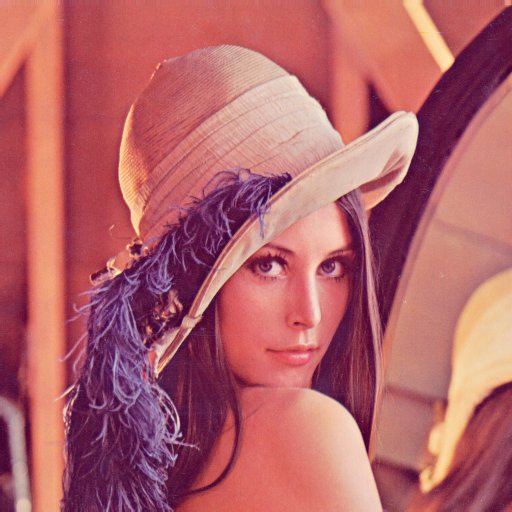
\includegraphics[scale=0.25]{lena.jpg}
\caption{Primer imagen utilizada para detecci\'on de bordes - lena.jpg}
\end{figure}

\vspace{3cm}

\begin{figure}[ht] %[h] para here [b] para bottom [t] para top
\centering
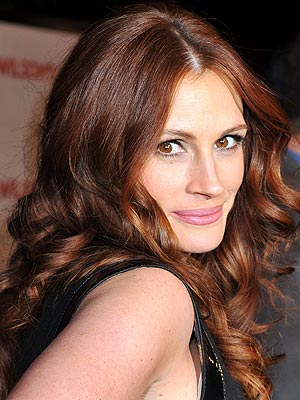
\includegraphics[scale=0.30]{roberts.jpg}\hspace{1cm}
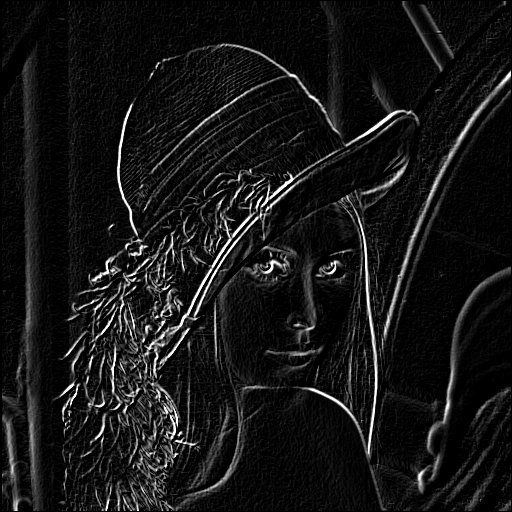
\includegraphics[scale=0.30]{prewitt.jpg}
\caption{Resultado de aplicar el operador Roberts y Prewitt para la imagen lena.jpg, respectivamente}
\end{figure}

\begin{figure}[ht] %[h] para here [b] para bottom [t] para top
\centering
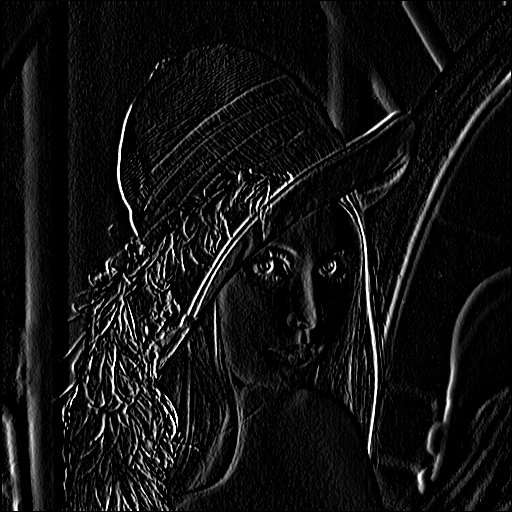
\includegraphics[scale=0.30]{sobelX.jpg}\hspace{1cm}
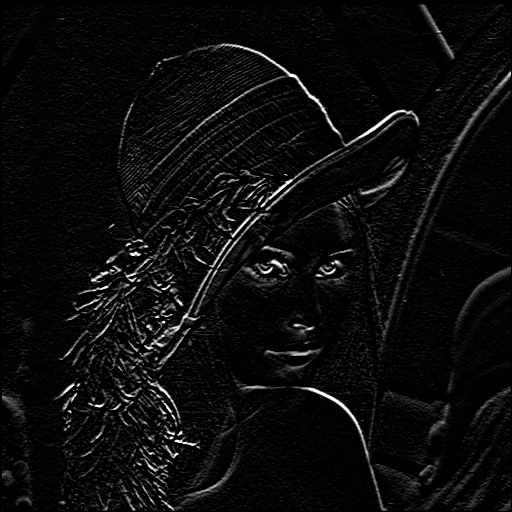
\includegraphics[scale=0.30]{sobelY.jpg}
\caption{Resultado de aplicar el operador sobelX y sobelY para la imagen lena.jpg, respectivamente}
\end{figure}
\vspace{5cm}
\begin{figure}[ht] %[h] para here [b] para bottom [t] para top
\centering
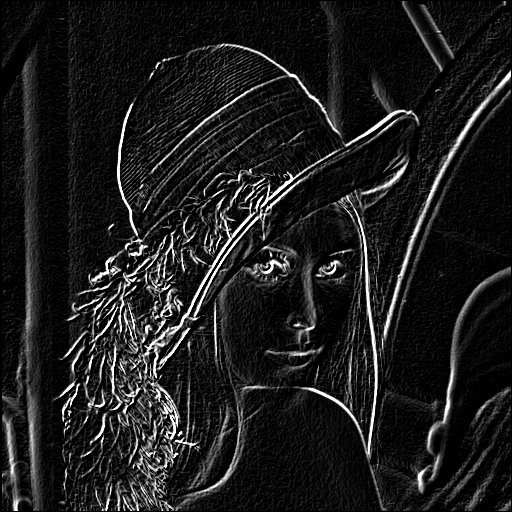
\includegraphics[scale=0.30]{sobelXY.jpg}
\caption{Resultado de aplicar el operador sobelXY para la imagen lena.jpg}
\end{figure}


\newpage
\section{Anexo Pseudoc\'odigos}
Pseudocodigo:

asmRoberts(src:char*, dst:char*, ancho:int ,alto:int,wstep:int)
{
	pSrc(ESI) 		$\leftarrow$	src; 			
	pDst(EDI) 		$\leftarrow$	dst;			
	filasFaltantes(ECX) 	$\leftarrow$	alto;		
	paso(EAX) 		$\leftarrow$	wstep;				
	limiteAncho(EDX) 	$\leftarrow$	ancho;					

	filasFaltantes(ECX)     $\leftarrow$ 	filasFaltantes(ECX) -1;
	limiteAncho(EDX) 	$\leftarrow$	limiteAncho(EDX) - 16;					
					

	do{
		pixelesProcesados(EBX) = 0;
	
		do{	
			if (ebx>edx) 

				pSrc(ESI) $\leftarrow$ pSrc(ESI) + limiteAncho(EDX) ;
				pSrc(ESI) $\leftarrow$ pSrc(ESI) - pixelesProcesados(EBX);
				
				pDst(EDI) $\leftarrow$ pDst(EDI) + limiteAncho(EDX) ;
				pDst(EDI) $\leftarrow$ pDst(EDI) - pixelesProcesados(EBX);
				
				procesar();
			else
			
				procesar();
	
		}while(ebx <= edx);
	
		pSrc(ESI) $\leftarrow$ pSrc(ESI) - limiteAncho(EDX);
		pSrc(ESI) $\leftarrow$ pSrc(ESI) + paso(EAX) ;
	
		pDst(EDI) $\leftarrow$ pDst(EDI) - limiteAncho(EDX);
		pDst(EDI) $\leftarrow$ pDst(EDI) + paso(EAX) ;
	
		filasFaltantes(ECX) $\leftarrow$ 	filasFaltantes(ECX) - 1; 
	
	}while(filasFaltantes(ECX) > 0); 
}	




procesar()
{
	xmm0 $\leftarrow$ [pSrc][127:0];
	xmm1 $\leftarrow$ [pSrc+paso][127:0];
	xmm2 $\leftarrow$ xmm0;
	xmm3 $\leftarrow$ xmm1;
	xmm3 $\leftarrow$ xmm3 >> 1;
	xmm2 $\leftarrow$ xmm2-xmm3;
	xmm0 $\leftarrow$ xmm0 >> 1;
	xmm0 $\leftarrow$ xmm0-xmm1;
	xmm0 $\leftarrow$ xmm0 + xmm2;
	xmm0 $\leftarrow$ xmm0 << 1;
	xmm0 $\leftarrow$ xmm0 >> 1;
	[pDst(EDI)][127:0] $\leftarrow$ xmm0;
}


\end{document} 
